%%%%%%%%%%%%%%%%%%%%%%%%%%%%%%%%%%%%%%%%%%%%%%%%%%%%%%%%%%%%%%%%%%%%%%%%%%%%%%%%
%2345678901234567890123456789012345678901234567890123456789012345678901234567890
%        1         2         3         4         5         6         7         8

\documentclass[letterpaper, 10 pt, conference]{ieeeconf}  % Comment this line out if you need a4paper

%\documentclass[a4paper, 10pt, conference]{ieeeconf}      % Use this line for a4 paper

\IEEEoverridecommandlockouts                              % This command is only needed if 
                                                          % you want to use the \thanks command

\overrideIEEEmargins                                      % Needed to meet printer requirements.

% See the \addtolength command later in the file to balance the column lengths
% on the last page of the document

% The following packages can be found on http:\\www.ctan.org
%\usepackage{graphics} % for pdf, bitmapped graphics files
%\usepackage{epsfig} % for postscript graphics files
%\usepackage{mathptmx} % assumes new font selection scheme installed
%\usepackage{times} % assumes new font selection scheme installed
%\usepackage{amsmath} % assumes amsmath package installed
%\usepackage{amssymb}  % assumes amsmath package installed
\usepackage{graphicx}
\usepackage[export]{adjustbox}
\usepackage{hyperref}
\graphicspath{ {images/} }


\title{\LARGE \bf
3D Object Modeling
}


\author{Pin-Wei Chen$^{1}$% <-this % stops a space
\thanks{*This work was supported by the Robotics Master Program in National Chiao Tung University, Taiwan}% <-this % stops a space
\thanks{$^{1}$Pin-Wei Chen, National Chiao Tung University, Taiwan.		{\tt\small ccpwearth@gmail.com}}%
}


\begin{document}



\maketitle
\thispagestyle{empty}
\pagestyle{empty}


\section{INTRODUCTION \& MOTIVATION}

Nowadays, people are using 3D information~\cite{vosselman20013d} more often to do their work than 2D information. For example: self-driving vehicle, model showing, object recongnition, identity reconginition, etc. As a result, building a 3D model becomes a significant issue and technology, the result can offer to many field.

I am going to use only one depth camera (SR-300) to build a 3D point cloud model of an object. The way I build the 3D model is to move the camera around the object, and get lots of point cloud for different view, finally, I will merge all point clouds from different views to build the 3D model.

\section{SYSTEM ARCHITECTURE \& EQUIPMENTS}

\subsection{SYSTEM ARCHITECTURE}

First, I use depth camera to recieve point cloud, and then I use TF to transform every point cloud to let their coordinate base on apriltags instead of camera link. Moreover, the way I get coordinate of apriltags is to use iSAM algorithm and get a more precise coordinate. And then, I use ICP~\cite{rusu20113d} (Iterative Closest Point) to merge each point cloud properly. After that, we can build a 3D point cloud model of the object. The system diagram shows in Fig.~\ref{figure:chart}.
\begin{figure}[h] % t means put this image here 

\includegraphics[width=1\columnwidth]{system_diagram}
\centering
\caption{3D object modeling flowchart}
\label{figure:chart}
\end{figure}

\subsection{EQUIPMENTS} 

For the hardware part, I use one depth camera (SR-300), which is connect to laptop, and I use several apriltags (36h11) to make the iSAM and TF work well. And then we need to put an object, which is going to be build a 3D model Fig.~\ref{figure:tissue}.

In software part, we use ROS kinetic, OpenCV 3.2.0 and ubuntu 16.04 LTS as our develop environment.

\begin{figure}[t] % t means put this image at the top 
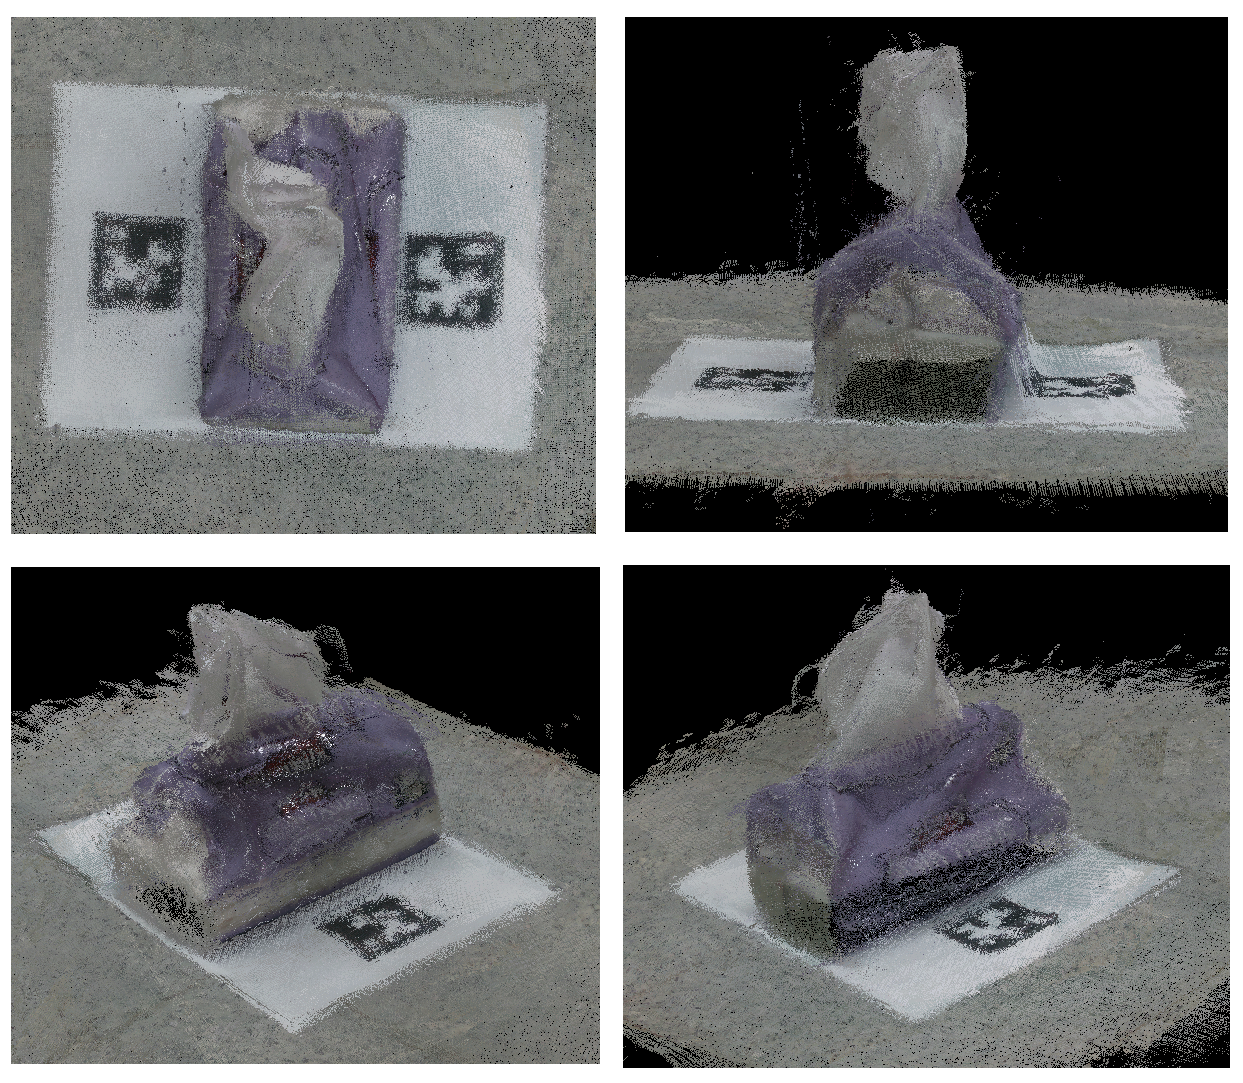
\includegraphics[width=0.8\columnwidth]{tissue}
\centering
\caption{3D object modeling}
\label{figure:tissue}
\end{figure}

\section{APPROACH}

\begin{itemize}
\item Using iSAM~\cite{kaess2008isam} to get a better performance of coordinate
\end{itemize}

I use several apriltags to get lots of coordinate informations, ant this can help to increase the amount of landmark for iSAM algorithm.

First, I fix every apriltags, and measure their relative position, and these relative position will become apriltags-apriltags pose3d parameters. Then I will use depth camera to capture all apriltags, getting the relative pose between camera link and apriltags, and these will become apriltags-camera pose3d parameters. At last, I add those relations, including apriltags-apriltags and apriltags-camera link, to iSAM pose3d factor, and call the function to optimize the coordinate, I will do this step once I get an point cloud from depth camera.

The aim of this step is to optimize the coordinate of apriltags, because the coordinate of apriltags only get from camera will have some errors, so I use iSAM to reduce the error.
\\
\begin{itemize}
\item Transfer coordinate by TF
\end{itemize}

TF is a library for ROS, and the function is to transfer the point cloud coordinate from camera link to apriltag, it can help us unify the coordinate from different view of point cloud.

The input of the TF is a point cloud and two frame, one is origin frame and another is target frame, and we can get the oput point cloud that have already transfer it coordinate from origin frame to target frame. 

The aims of this step is to let every point cloud base on the same frame, so that all point clouds can approximately match together.
\\
\begin{itemize}
\item Merge point clouds using ICP
\end{itemize}

The coordinate of apriltags generate from iSAM will still have some error, so that the point cloud will not match with each other prcisely, so I use ICP to help merge each point cloud together perfectly.

ICP is the abbreviation of "Iterative Closet Point", this library can use iteration to rotate and translate one point cloud to match another point cloud.
\\
\begin{itemize}
\item Build a 3D object model into PCD file
\end{itemize}

After merging all the point cloud, I can get the 3D model of the object, and I save it as an PCD file, so that others can use this model conveniently, moreover, there are lots of library and editor such as PCD editor which can adjust and edit the point cloud easily.

\section{RESULT}

\begin{itemize}
\item Untreated Point Cloud
\end{itemize}

The original untreated point cloud is generated by adding the whole point cloud directly, however, every point cloud base on different frame, so the result will be pretty messy Fig.~\ref{figure:untreated}.

\begin{figure}[h] % t means put this image here 
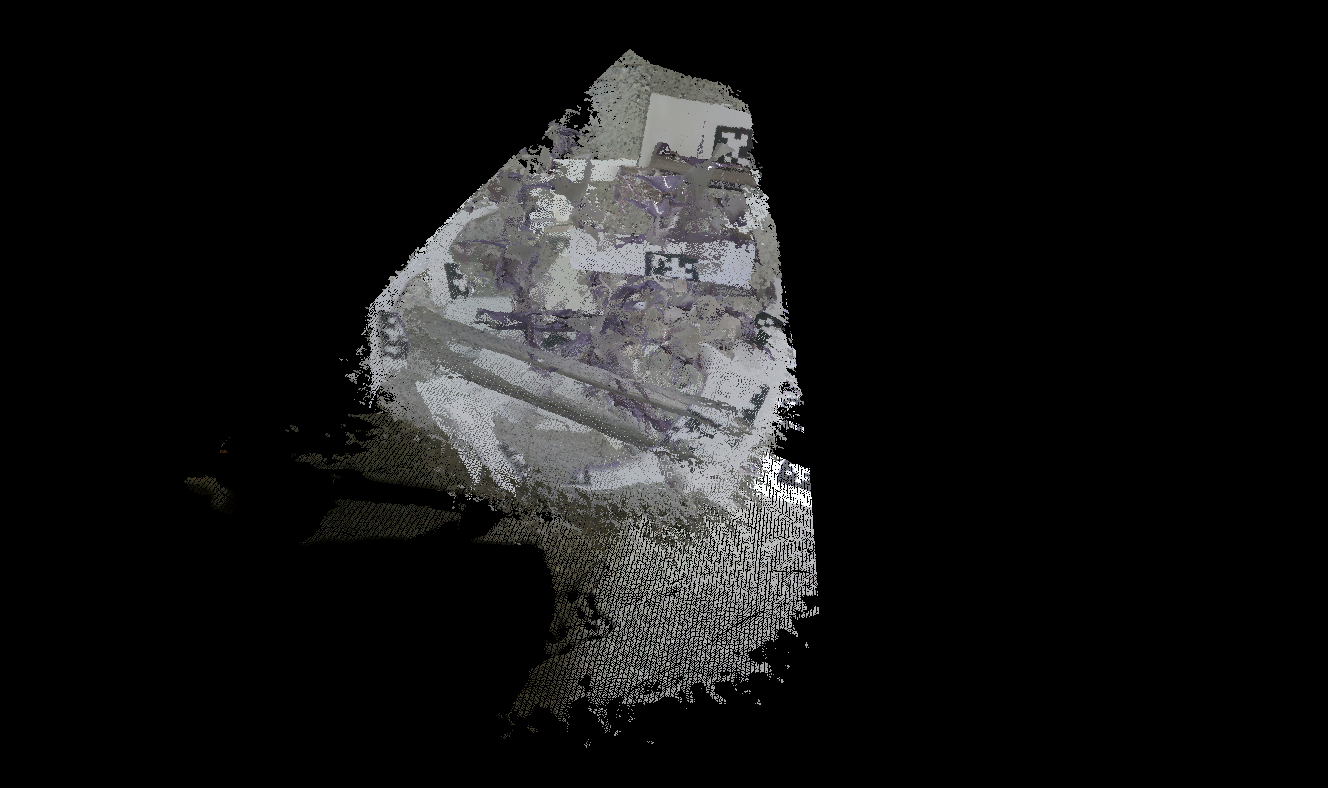
\includegraphics[width=0.8\columnwidth]{add}
\centering
\caption{Untreated Point Cloud}
\label{figure:untreated}
\end{figure}

\begin{itemize}
\item Using TF
\end{itemize}

The result of using TF looks much more better then untreated one, because every point cloud have already base on same frame, apriltags ID: 1, so that they can match approximately, however, the coordinate of the apriltags still have some error, so they still can't match perfectly Fig.~\ref{figure:TF}.

\begin{figure}[h] % t means put this image here 
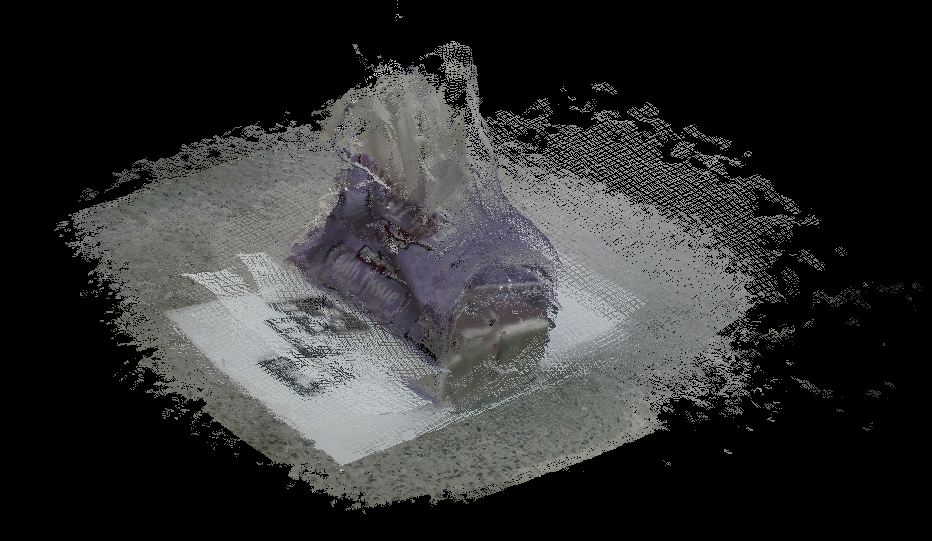
\includegraphics[width=0.8\columnwidth]{tf}
\centering
\caption{Using TF}
\label{figure:TF}
\end{figure}

\begin{itemize}
\item Using ICP
\end{itemize}

When only use ICP to merge the point cloud, it takes a very long time to finish the merge of two point clouds. It is because the two point clouds are base on two different coordinates, the ICP algorithm need lots of iterations and caculations to merge the two point clouds. As a result, during the limited time, the final result of only using ICP can merge will but lack of points, due to the long caculation time. Fig.~\ref{figure:ICP}.

\begin{figure}[h] % t means put this image here 
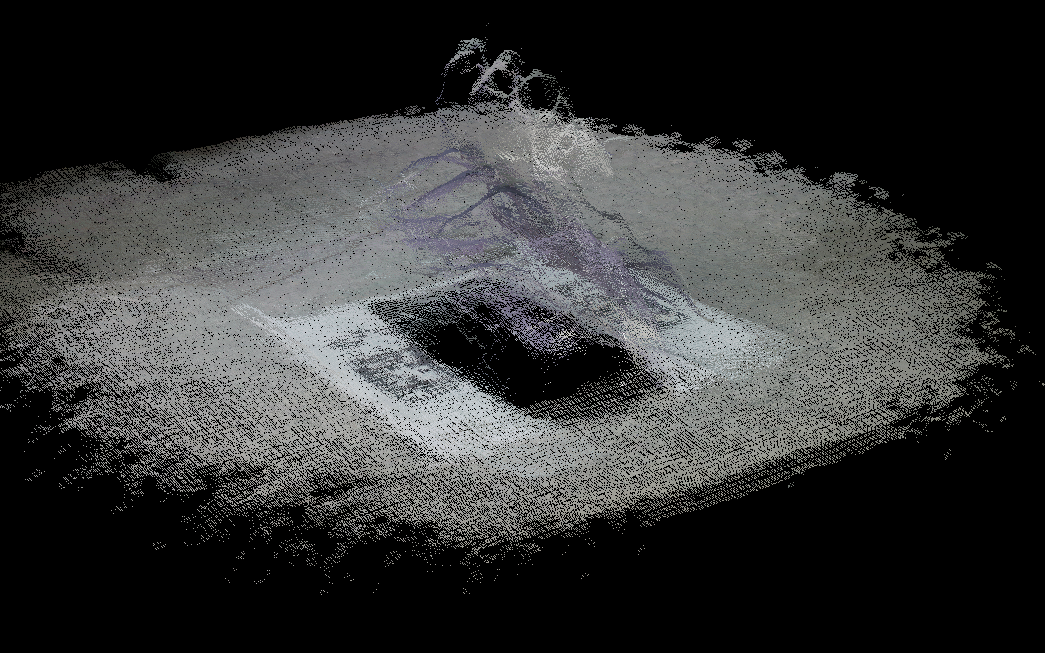
\includegraphics[width=0.8\columnwidth]{icp}
\centering
\caption{Using ICP}
\label{figure:ICP}
\end{figure}

\begin{itemize}
\item Using TF + ICP + iSAM
\end{itemize}

Combining the result of above, I use TF and ICP together to improve the performance, and I also use iSAM algorithm to optimize the apriltags coordinate. The result of Using TF + ICP + iSAM is pretty satisfying. 

Now, it can merge more precisely then only using TF. Moreover, it has more points then only using ICP, because the whole point clouds have already using TF to base on the same coordinate, the ICP caculation time and iteration will reduce significantly. As a result, I can get a result that has perfect merging and enough points to see the details of the object Fig.~\ref{figure:iSAM}.

\begin{figure}[h] % t means put this image here 
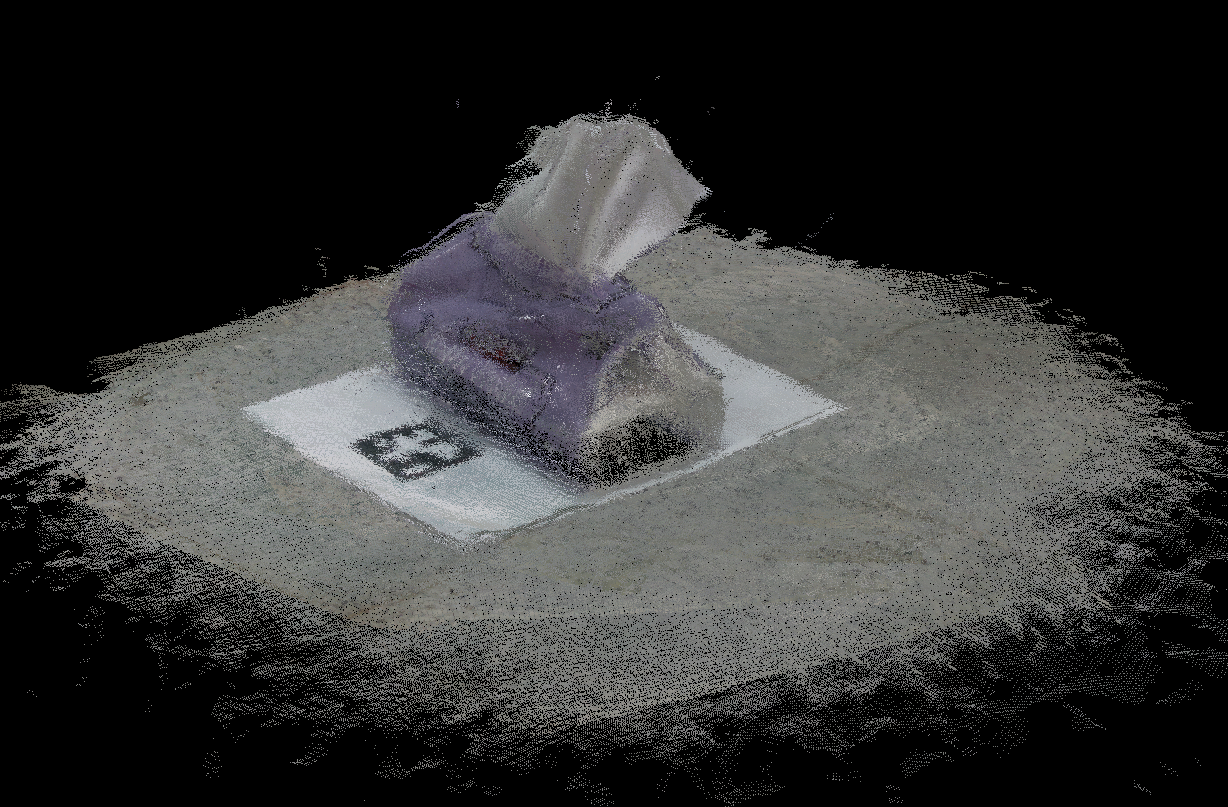
\includegraphics[width=0.8\columnwidth]{iSAM}
\centering
\caption{Using ICP}
\label{figure:iSAM}
\end{figure}

\section{CONCLUSION}

We can see the comparasion table in Fig.~\ref{figure:compare}, the calculation time TF works the best, cause it doesn't really need any caculation, the only caculation is the transform of the coordinate, and the worst case is using only ICP, because it needs lots of iterations. 

For the Integrity, the worst case is using only ICP, because it need lots of caculation time and iterations, so it will lack of points, making lots of details of object been disappear. The best case is using TF + ICP + iSAM.

For the accuracy, the best case is using TF + ICP + iSAM, because it transfer the coordinate and also use ICP to merge the point cloud, and the worst case is using only TF, because the error of apriltags will always exist.

In conclusion, the best performance is to use TF + ICP + iSAM, it can generate a complete point cloud model which is been merge pretty well.

\begin{figure}[h] % t means put this image here 

\includegraphics[width=1\columnwidth]{compare}
\centering
\caption{Comparasion}
\label{figure:compare}
\end{figure}



\addtolength{\textheight}{-12cm}   % This command serves to balance the column lengths
                                  % on the last page of the document manually. It shortens
                                  % the textheight of the last page by a suitable amount.
                                  % This command does not take effect until the next page
                                  % so it should come on the page before the last. Make
                                  % sure that you do not shorten the textheight too much.

\bibliographystyle{IEEEtran}
\bibliography{egbib}

\end{document}